\documentclass[10pt, a4paper]{article}

\usepackage{graphicx}
\usepackage{changepage}
\usepackage[rightcaption]{sidecap}
\usepackage{hyperref}

\title{Rapport bibliographique : Modélisation et fabrication d’un actionneur pneumatique souple}
\author{Loïc Mosser, Master IRIV, Parcours IRMC}
\date{Avril 2020}

\begin{document}

\makeatletter

    \begin{titlepage}
    
        \begin{center}
             
            \begin{figure}[!htb]
            \begin{adjustwidth}{-3cm}{-3cm}  
               \begin{minipage}{0.30\textwidth}
                 \centering
                 
\includegraphics[width=1\linewidth]{Logo/Icube.png}
                 
               \end{minipage}\hfill
               \begin{minipage}{0.30\textwidth}
                 \centering
                 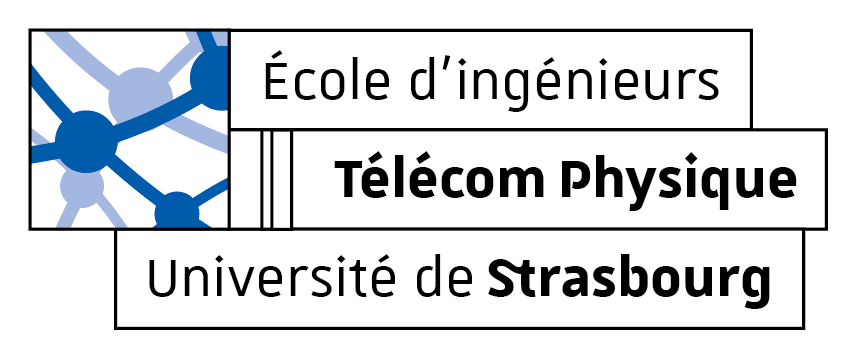
\includegraphics[width=1\linewidth]{Logo/TPS.png}
               \end{minipage}\hfill
               \begin{minipage}{0.30\textwidth}
                 \centering
                 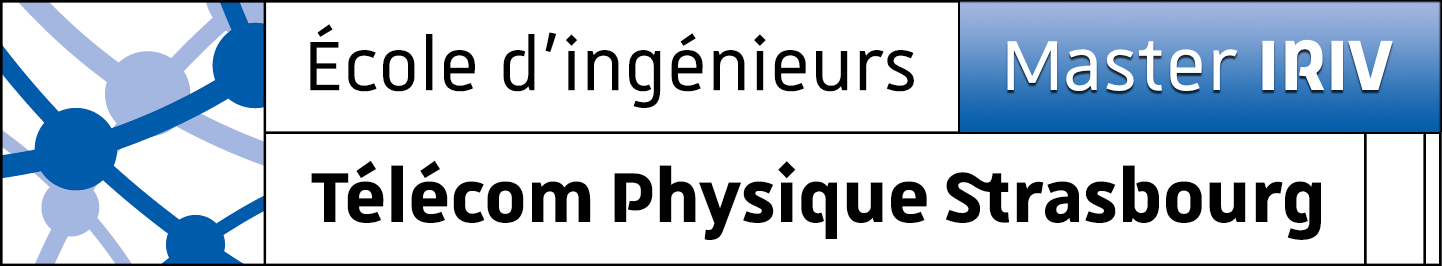
\includegraphics[width=1\linewidth]{Logo/IRIV.png}
               \end{minipage}\hfill
               \begin{minipage}{0.30\textwidth}
                 \centering
                 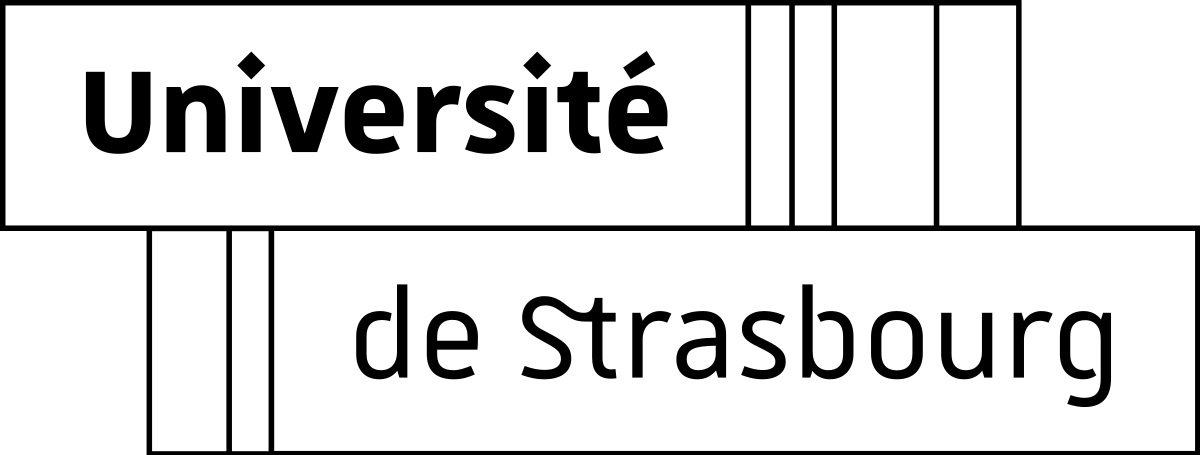
\includegraphics[width=1\linewidth]{Logo/Strasbourg.svg.png}
               \end{minipage}
               \end{adjustwidth}
            \end{figure}
            

            {\huge \bfseries  \@title }\\[15ex] 
            {\LARGE  \@author}\\[10ex] 
            {\large  Encadrants :}\\[2ex] 
            {\large  Pierre Renaud}\\[2ex] 
            {\large  Laurent Barbé}\\[2ex] 
            {\large  François Geiskopf}\\[17ex] 
            
            {\large \@date}
        \end{center}
        
    \end{titlepage}
\makeatother
\thispagestyle{empty}
\newpage

%Add content for page two here (useful for two-sided printing)
%\thispagestyle{empty}
%\newpage
%\maketitle
%\setcounter{page}{1} %Start the actually document on page 1

\tableofcontents
\newpage

\section{Introduction}
    \subsection{Intérêt de l'actionnement linéaire dans le cadre de l'IRM}
    
     L'Imagerie par Résonance Magnétique (IRM, figure \ref{fig:IRM}) est un dispositif d'imagerie médicale couramment utilisée pour le diagnostique et le suivi de traitement chez des patients atteints de cancers notamment. Elle utilise un champ magnétique fixe de l'ordre du tesla et un champ tournant pour obtenir des images. La place dans ces dispositifs médicaux est restreinte à cause de la difficulté qu'ont les concepteurs à garder le champ fixe constant dans le tunnel. Tout dispositif tiers devient alors contraint à un espace réduit s'il souhaite opérer dans le tunnel d'un IRM. \\


\begin{figure}[ht!]
\centering
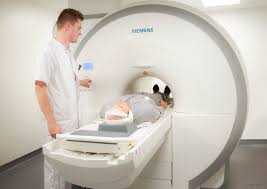
\includegraphics[scale=1]{ImageIntro/IRM.jpg}
\caption{Image d'un dispositif d'IRM avec un opérateur et un patient qui s'apprête à subir un examen (source : \url{http://www.angers-radiologie.fr/examen-radiologique/irm/}) }
\label{fig:IRM}
\end{figure}


    Il est possible d'utiliser ce dispositif avec d'autres qui tiennent compte des contraintes de taille et de compatibilité IRM, comme des stimulateur pneumatiques, pour mesurer des grandeurs secondaires comme le module de cisaillement des tissus mous. C'est le cas de l'élastographie par résonance magnétique \cite{Ehman2012} par exemple (figure \ref{fig:ERM}).\\
    
    
\begin{figure}[ht!]
\centering
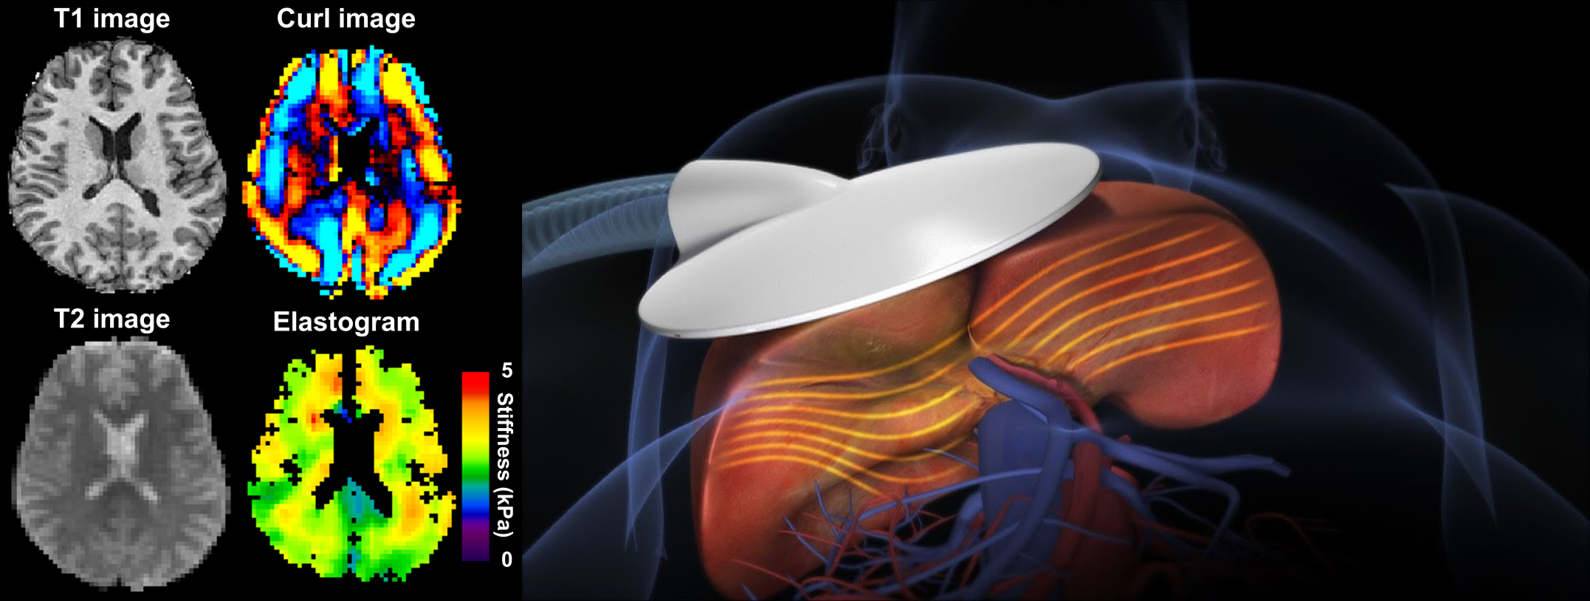
\includegraphics[scale=0.4]{ImageIntro/ERM.png}
\caption{Image du dispositif d'ERM avec son palpeur (à droite) et les image ainsi obtenues (à gauche) (sources : \url{https://en.wikipedia.org/wiki/Magnetic_resonance_elastography} et \url{https://www.youtube.com/watch?v=CcmZi0J_u3Y)}}
\label{fig:ERM}
\end{figure}

Il est maintenant possible d'envisager l'utilisation de cette modalité d'imagerie pour guider un geste médical comme le prélèvement d'échantillon biologiques \cite{Cleary2018}. En effet, dans la mesure où les prélèvements biologiques de corps profondément enfuis sont incertains, un guidage par IRM permet de réduire le risque de prélèvement dangereux et non pertinents \cite{Cleary2018}. L'insertion d'aiguille, et l'actionnement en milieu IRM plus généralement, devient alors un besoin médical.\\

Effet, d'autres actionnement avec des caractéristiques cinématique différentes peuvent être nécessaire pour des gestes comme la palpation \cite{Moerman2013} ou encore le guidage de HIFU(High-Intensity Focused Ultrasound) sous IRM \cite{Melzer2008}\cite{Wang2019}. Elles mettent en jeu des problématiques d'actionnement différentes. Néanmoins, les problématiques restent les mêmes quelque soient les actionnements envisagées du point de vue de la compatibilité IRM.
    
    \subsection{Problématique associée}
    
 L'introduction de composants dans le tunnel d'un IRM peut poser plusieurs difficultés. Tout d'abord, tout corps ferro-magnétique est proscris en IRM \cite{Sammet2016}, il est nécessaire de s'assurer que le corps introduit n'induise pas d'artefacts de mesure par l'IRM \cite{Sammet2016} (figure \ref{fig:IRM-Artefact}). En effet, certains matériaux pouvant déformer le champ fixe par leurs présence, la mesure et la reconstruction effectuée dans la traitement ne pourra pas être effectuée correctement. Le composant introduit dans l'IRM doit donc prévoir cet aspect du milieu dans lequel il évolue. De plus, à cause des éventuelles boucles présentes dans le système, des courants induits peuvent poser des problèmes d'échauffement dans l'appareil d'imagerie \cite{Sammet2016}.


\begin{figure}[ht!]
\centering
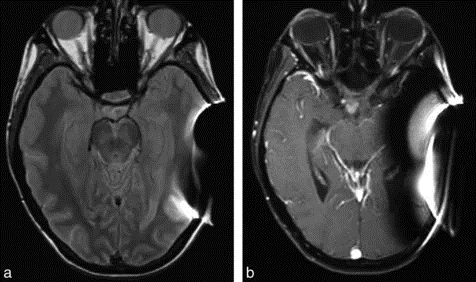
\includegraphics[scale=0.5]{ImageIntro/artefacts.png}
\caption{Artefact dans une image issue d'un IRM causée par un objet métallique non ferro-magnétique (source : \url{https://clemedicine.com/11-artefacts-en-imagerie-par-resonance-magnetique/} ) }
\label{fig:IRM-Artefact}
\end{figure}
    
\section{Système actuel} 

    \subsection{Architecture}
    
\begin{figure}[ht!]
\centering
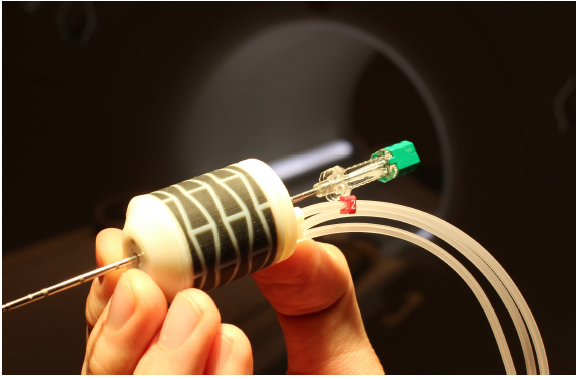
\includegraphics[scale=0.5]{ImageIntro/Inchworm.PNG}
\caption{ Système Actuel (source : \cite{Pfeil2018})}
\label{fig:Inchworm}
\end{figure}   

         Actuellement, un actionneur linéaire pneumatique, dédié à l'insertion d'aiguille, a déjà été développé au sein de l'équipe AVR du laboratoire Icube \cite{Pfeil2018}. Le système épouse l'aiguille pour un guidage précis et complet (figure \ref{fig:Inchworm}). Il se décompose en trois parties: deux mors de serrage (MG et FG dans la figure \ref{fig:planInchworm}) et une chambre auxétique(MC dans la figure \ref{fig:planInchworm}). Ces trois parties permettent l'actionnement inchworm (figure \ref{fig:planInchworm}) par l'actionneur sur l'aiguille. Ce fonctionnement est décrit en partie 3.2.2. Les trois parties sont alimentées en énergie pneumatique de manière indépendantes pour assurer ce fonctionnement. 
        
\begin{figure}[ht!]
\centering
\includegraphics[scale=0.7]{ImageIntro/SéquenceInchworm.PNG}
\caption{ Schéma de la séquence permettant l'actionnement inchworm (source : \cite{Pfeil2018})}
\label{fig:planInchworm}
\end{figure}
        
    \subsection{Matériaux et procédé}

         Actuellement, le système est réalisé par fabrication additive bi-matériaux avec la technologie polyjet \cite{Pfeil2018} (figure \ref{fig:fabPoly}). La pièce est donc fabriquée à l'aide d'un dépôt de photopolymère dont la polymérisation est réalisée grâce au passage d'une lampe UV. Le dépôt successif de matière permet la polymérisation de la première couche et des couches précédentes. L'utilisation d'un matériau de support qui peut être supprimer grâce à une étape supplémentaire, comme le bain de soude, permet la fabrication de formes particulière comme des cavités et des renfoncements profonds. D'autres procédés comme l'usinage ou le moulage en seraient incapables à cause de leurs contraintes propres. Ce procédé est très adapté aux fabrication de petites séries de pièces, à cause des temps long de mise en forme, et au développement de nouvelles applications. 
        
\begin{figure}[ht!]
\centering
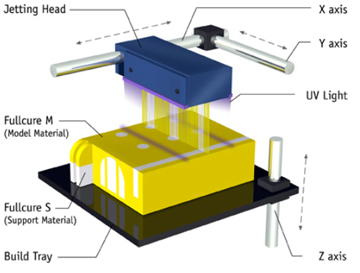
\includegraphics[scale=0.5]{ImageIntro/polyjet_process2.jpg}
\caption{ Illustration du procédé de fabrication utilisé pour réaliser le système original (source : \url{https://www.a3dm-magazine.fr/news/fabrication-additive-polymeres/procede-dimpression-3d-polyjet-jet-dencre})}
\label{fig:fabPoly}
\end{figure}        

    \subsection{Structure auxétique}
    
         Une des composantes du système permet l'avance de l'aiguille, c'est la chambre auxétique (figure \ref{fig:maillageAux}). Cette chambre est composée d'un élastomère, le tangoBlackPlus (source : https://www.stratasys.com/materials/search/tango), renforcée par un squelette en plastique rigide (Module d'Young de 2 GPa (source : https://www.stratasys.com/materials/search/vero))  avec une maille élémentaire qui donne à la chambre sa propriété auxétique \cite{Karnessis2013}. Cette chambre possède un coefficient de poisson négatif ce qui lui permet de s'allonger lorsque qu'une pression est appliquée à l'intérieur de celle-ci. Cela ce rapproche de certains méta matériaux avec des propriétés impossibles à avoir de manière naturelles, ce sont pour la plupart des mousses synthétiques \cite{Ashby1983}. 
        
\begin{figure}[ht!]0
\centering
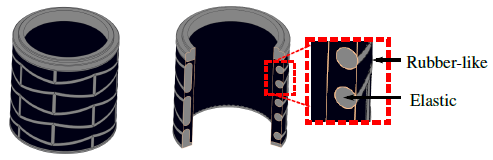
\includegraphics[scale=0.8]{ImageIntro/mailleAux.PNG}
\caption{ Représentation 3D de la chambre auxétique avec le maillage en matériaux rigide et de l'enveloppe en élastomère (source : \cite{Pfeil2018}) }
\label{fig:maillageAux}
\end{figure} 
        
    \subsection{Préhension}
        \qquad Le maintient de l'aiguille est permis par deux mors (figure \ref{fig:mors}) reliés entre eux par la chambre auxétique. Ces mors peuvent assurer un effort appliqué sur l'aiguille de 5N (rapport d'étude interne) sous une pression de 2 bars. La pression
        
\begin{figure}[ht!]
\centering
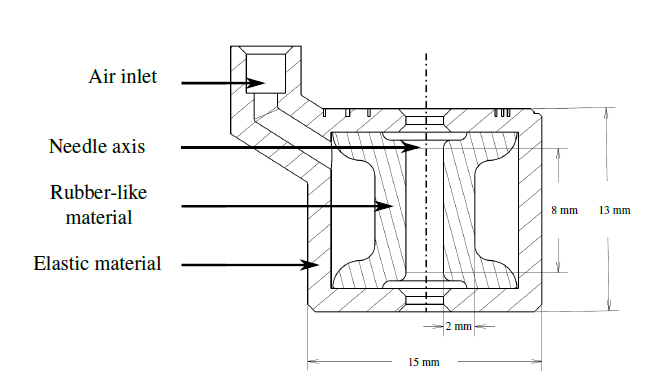
\includegraphics[scale=0.5]{ImageIntro/mors.PNG}
\caption{ Schéma plan d'un mors utilisé dans le système (source : \cite{Pfeil2018})}
\label{fig:mors}
\end{figure} 

\section{Technologie d'actionnement Linéaire dans le cadre de l'IRM}

    \qquad Dans le cadre de l'actionnement en milieu IRM, différentes technologies d'actionnements peuvent être utilisées. Néanmoins, la littérature scientifique dans le domaine \cite{Fischer2008} se focalise sur trois sortes d'actionnement : l'actionnement pneumatique \cite{Pfeil2018}\cite{Fischer2008a}, ultrasonique \cite{Masamune1995} et piézoélectrique \cite{Wang2009}\cite{Su2015}\cite{Su2012}. Les deux derniers sont regroupés dans la même sous catégorie car ils présentent des caractéristiques similaires.
    
    \subsection{Type d'actionnement}
        \subsubsection{Actionnement piézoélectrique/ultrasonore}
        
             \qquad La conversion d'énergie effectué dans les deux cas est différentes. Un actionneur piézoélectrique convertit de l'énergie électrique en énergie mécanique (figure \ref{fig:actPiUl} gauche) et un actionneur ultrasonique convertit de l'énergie mécanique en énergie mécanique. Néanmoins, la création des ultrasons, dans le cadre de l'actionnement ultrasonore, est réalisée grâce à des éléments piézoélectrique \cite{Masamune1995} (figure \ref{fig:actPiUl} droite) qui eux même convertissent l'énergie électrique en énergie mécanique.
            
\begin{figure}[ht!]
\centering
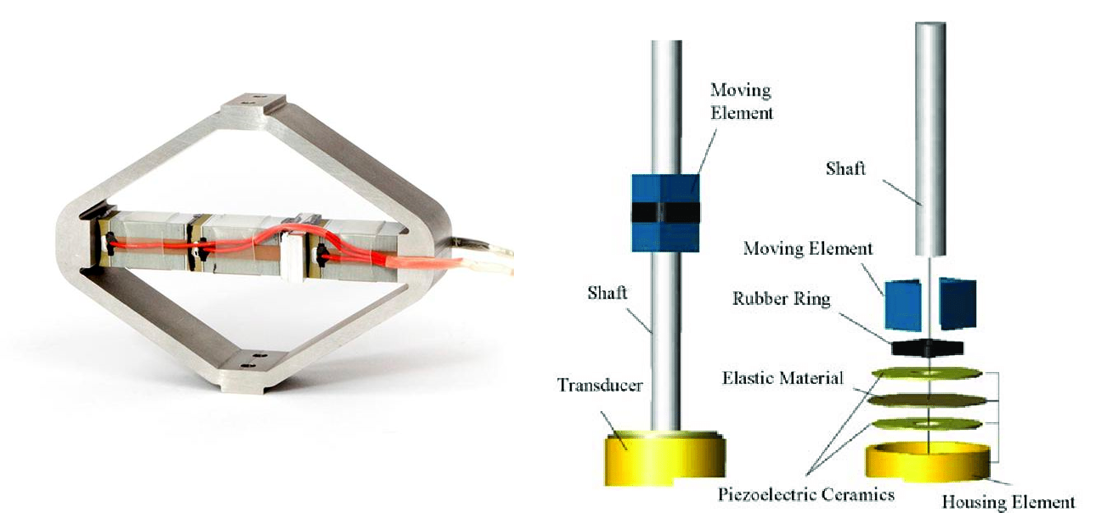
\includegraphics[scale=0.5]{ImageIntro/ActPizeUltr.png}
\caption{ Exemple d'actionneur piézoélectrique et d'actionneur ultrasonore (source: \url{https://www.directindustry.fr/prod/cedrat-technologies/product-54728-1461955.html} et \url{https://www.researchgate.net/figure/Fabricated-TULATiny-ultrasonic-linear-actuator_fig1_260594716}) }
\label{fig:actPiUl}
\end{figure} 
            
            \justify L'actionnement piézoélectrique peut être utilisé de deux manières: en générateur de forces et de petits déplacements \cite{Li2005} et en système pas à pas \cite{Su2012}\cite{Su2015}\cite{Wendt2000}. Dans le premier cas, la tension appliquée permet d'engager une déformation que l'on exploite directement pour l'actionnement. Dans le second, l'excitation du quartz et son architecture permet de mettre en mouvement l'effecteur grâce à une succession de petites déformations qui forment, à l'échelle microscopique, un système pas à pas (figure \ref{fig:indenteur}). C'est le même fonctionnement pas à pas utilisé pour les actionneurs ultra-sonores. Les ondes mécaniques viennent exciter un matériau avec cette architecture spécifique et cela engendre un mouvement.
            
\begin{figure}[ht!]
\centering
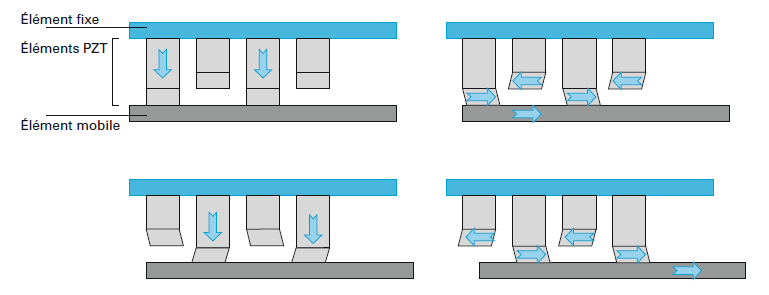
\includegraphics[scale=0.5]{ImageIntro/Indenteur.PNG}
\caption{ Principe de fonctionnement des actionneurs piézoélectriques et ultra-sonores (source : \cite{Lambert2016})}
\label{fig:indenteur}
\end{figure} 

         Ces actionnement ont néanmoins des défauts. L'apport nécessaire d'énergie électrique est une tâche complexe et coûteuse à réaliser en milieu IRM \cite{Su2012}. En effet, le boîtier de commande et d'alimentation électrique est en communication via une fibre optique avec la salle de commande de l'IRM et celui-ci possède un blindage pour éviter la pollution électromagnétique de l'IRM sur les cartes des (Figure \ref{fig:CommandePiezo}). De plus l'usage de ces technologies induisent des artefacts dans l'image reconstruite par l'imageur \cite{Wendt2000}.
        
\begin{figure}[ht!]
\centering
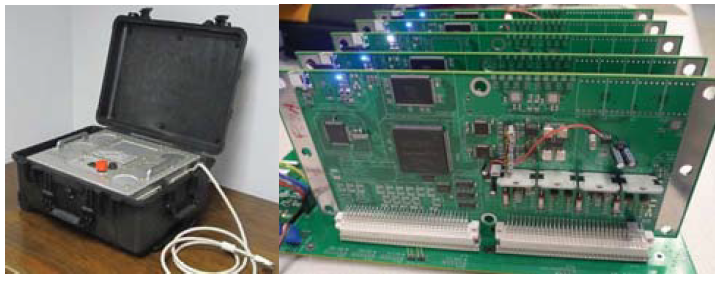
\includegraphics[scale=0.5]{ImageIntro/CommandePiezo.PNG}
\caption{ Boîtier de commande d'actionneurs piézoélectriques (source : \cite{Su2012})}
\label{fig:CommandePiezo}
\end{figure} 
            
        \subsubsection{Actionnement fluidique}
        
            \qquad L'actionnement fluidique comprend l'actionnement par voie pneumatique et par voie hydraulique. L'actionnement pneumatique est déjà couramment utilisé dans l'actionnement IRM car son utilisation ne nécessite pas de dispositions aussi lourde que pour l'utilisation de l'énergie électrique. L'énergie pneumatique peut être amenée à l'actionneur par des flexible depuis un contrôleur pneumatique se situant à distance de l'IRM \cite{Fischer2008a}\cite{Pfeil2018}. 
            
             L'actionnement hydraulique n'est pas un actionnement envisagé par la communauté scientifique \cite{Fischer2008}. L'actionnement hydraulique permet de développer des effort bien plus important que dans le cadre d'actionnement pneumatique et est plus contraignant en cas de fuite et dans sa maintenance. Les efforts à mettre en oeuvre sont trop faibles \cite{Pfeil2018}\cite{Fischer2008a} pour mettre en oeuvre un actionnement hydraulique. De plus, l'actionnement hydraulique nécessite d'avoir des matériaux rigide et capable de tenir de fortes pressions, or tout métal para-magnétique ou dia-magnétique ainsi que ferro-magnétique est proscrit du milieu IRM pour ne pas brûler ou blesser le patient \cite{Sammet2016}.
             
 
             L'actionnement fluidique a donc de nombreux avantages pour l'actionnement en milieu IRM. Il est, de plus, possible d'envisager des actionnements particuliers et non conventionnelles grâces à des structures souples dont des cavités mises sous pressions (figure \ref{fig:ActSouple}) permettent une articulation le long d'une ligne quelconque par exemple . \cite{Lambert2016}\cite{Sedal2018}\cite{Lazarus2017}\cite{Sedal2018a}\cite{Polygerinos2015}\cite{Connolly2017}. 
             
\begin{figure}[ht!]
\centering
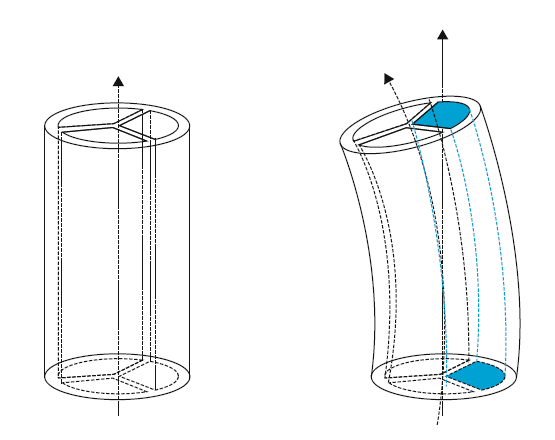
\includegraphics[scale=0.4]{ImageIntro/ExemplaActionnementSouple.PNG}
\caption{ Exemple d'actionneur pneumatique souple (source : \cite{Lambert2016})}
\label{fig:ActSouple}
\end{figure}
             
    \subsection{Génération de mouvement}
    
        \qquad Étant donné ces différentes formes d'énergies et d'actionnements possibles, deux grandes classes de systèmes apparaissent. Il existe des systèmes qui exploitent directement la mobilité offerte par l'actionneur pour mettre en mouvement des effecteurs. D'autres exploitent plusieurs actionnement pour mettre en place un fonctionnement pas à pas.
        
        \subsubsection{Actionnement continu}
        
            \qquad Afin de générer un mouvement continu linéaire, plusieurs solutions existent. Certaines exploitent un actionnement en rotation. C'est le cas de la transmission roue/ vis sans fin et pignon crémaillère. Par exemple, des systèmes roue/vis sans fin sont mis en place pour l'actionnement linéaire sur trois axes pour former une plateforme capable de ce déplacer sur les trois axes cartésiens \cite{Su2012}. De même, la liaison pignon/crémaillère est utilisé dans l'actionnement linéaire de systèmes compatibles IRM \cite{Kanayama2019} (figure \ref{fig:stimIRM}).
            
\begin{figure}[ht!]
\centering
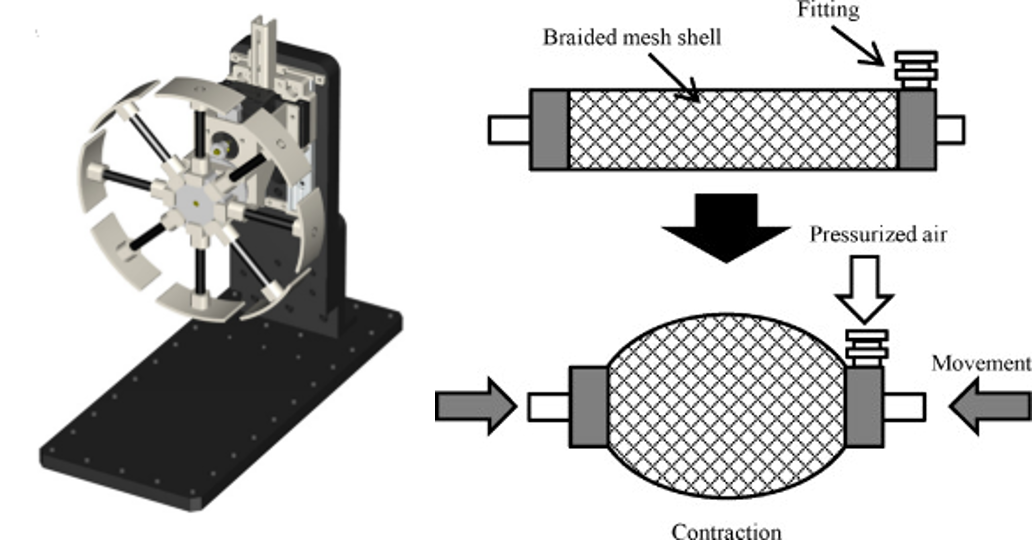
\includegraphics[scale=0.5]{ImageIntro/pignoncremMackibben.png}
\caption{ Stimulateur tactile IRM compatible avec une liaison pignon/crémaillère et schéma de principe du muscle artificiel de mac Kibben (source : \cite{Kanayama2019} , \cite{Takashima2010})}
\label{fig:stimIRM}
\end{figure}
            
            D'autres systèmes permettent des actionnements linéaire qui ne dépendent pas de rotations comme le muscle artificiel de mac kibben \cite{Lambert2016}\cite{Zhang2012}\cite{Daerden2002}\cite{Chou1996}\cite{Doumit2009} (figure \ref{fig:stimIRM}) qui se rapproche ,dans ses mobilités, d'un vérin pneumatique mono-stable. Le système se sert de la compression d'une chambre renforcée par un tissu avec une maille oblique pour réduire sa taille et ainsi générer un effort.
             
        \subsubsection{Inchworm et systèmes pas à pas}
        
    D'autres actionnements comme le fonctionnement inchworm exploitent plusieurs actionnements pour mettre en place un actionnement pas à pas. C'est le cas du fonctionnement Inchworm vu en section 2.1 (figure \ref{fig:Inchworm}). Celui-ci exploite trois actionnement pneumatique. Deux permettent la préhension de l'effecteur à mettre en mouvement et un troisième permet le mouvement en lui-même.Plus généralement, ce fonctionnement a des avantages comme le fait que sa course ne soit limité que par la longueur de l'effecteur. Des systèmes plans avec un fonctionnement inchworm \cite{Zhou2020} existent. De même, des actionneurs inchworms en rotations ont déjà été imaginés et utilisés \cite{Sun2015} \cite{Song2018}. Cet méthode d'actionnement peut être utilisée à des échelles très différentes \cite{Hochwallner2017}. Les actionneur inchworms peuvent, de plus, utiliser toutes sortes d'énergies : magnétiques (incompatible IRM) \cite{Zhou2020} \cite{Kim2002}, piézoélectrique \cite{Song2018} \cite{Li2005} \cite{Sun2015} et pneumatique \cite{Mark2016} \cite{Pfeil2018}. Il est aussi envisageable de réaliser cet actionnement avec une redondance des axes à actionner \cite{Landberg2017} pour permettre des charges bien plus importantes (figure \ref{fig:multipleinchworm}).
    
    Certains actionnements Inchworm pas à pas ne sont pas réaliser sur des éléments "lisses" comme des cylindres ou des plans mais sur des éléments similaires à des crémaillères. En effet, alors que la plupart des actionneurs inchworms utilisent des mors lisses pour maintenir, par adhérence, l'effecteur \cite{Pfeil2018} \cite{Song2018} \cite{Li2005} \cite{Zhou2020} \cite{Sun2015}, d'autres réalisent une préhension par obstacle \cite{Groenhuis2016} \cite{Groenhuis2016a}. Cela signifie que les mors dentés viennent se figer dans une crémaillère lors du maintient.
            
\begin{figure}[ht!]
\centering
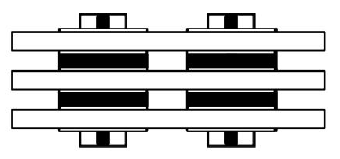
\includegraphics[scale=0.5]{ImageIntro/multipleInch.PNG}
\caption{ Schéma d'un fonctionnement inchworm sur plusieurs lignes (source : \cite{Landberg2017})}
\label{fig:multipleinchworm}
\end{figure}

\section{Méta matériaux} 

    Une définition en vigueur pour le terme de méta matériaux est " un matériau composite macroscopique et tridimensionnel, conçu par l'Homme avec une architecture périodique et en vue d'obtenir une combinaison optimisée de deux ou plusieurs réponses à une excitation spécifique" (source : https://www.futura-sciences.com/sciences/definitions/metamateriaux-metamateriau-4437/). Les structures auxétiques et les chambres renforcées par fibres rentrent dans cette définition. Elles sont, de plus, largement utilisées dans la littérature scientifique \cite{Doumit2009} \cite{Chou1996} \cite{Sedal2018} \cite{Sedal2018a} \cite{Lazarus2017} \cite{Takashima2010} \cite{Connolly2017} \cite{Polygerinos2015} \cite{Mark2016} \cite{Bruyas2016} \cite{Pfeil2018}. 
    
    
    \subsection{Structure Auxétique}
    
    Les structures auxétiques sont des architectures avec un coefficient de poisson négatif. Cela signifie qu'une telle structure se dilate si elle subit une élongation et inversement. Son comportement est dû à la géométrie de maille élémentaire. En effet, son architecture n'est que la répétition d'une maille élémentaire. Il est possible de trouver un grand nombre de tel motif dans la littérature scientifique (figure ) : nid d'abeille renversé \cite{Sedal2018} \cite{Alderson2007} \cite{Schumacher2018} \cite{Naboni2015} \cite{Lakes1991} \cite{Karnessis2013} \cite{Simons2019} \cite{AlvarezElipe2012} (figure \ref{fig:maillesAux} C et D), en sinusoïde ré-entrant \cite{Simons2019} \cite{Naboni2015} \cite{AlvarezElipe2012} (figure \ref{fig:maillesAux} A et B (version modifiée pour la photo B)), en double pointe de flèche \cite{Alderson2007} \cite{Karnessis2013} \cite{AlvarezElipe2012}, etc (figure ). Ces motifs donnent à la structure, qui contient une répétition de ceux-ci, des propriétés auxétiques. 
    
\begin{figure}[ht!]
\centering
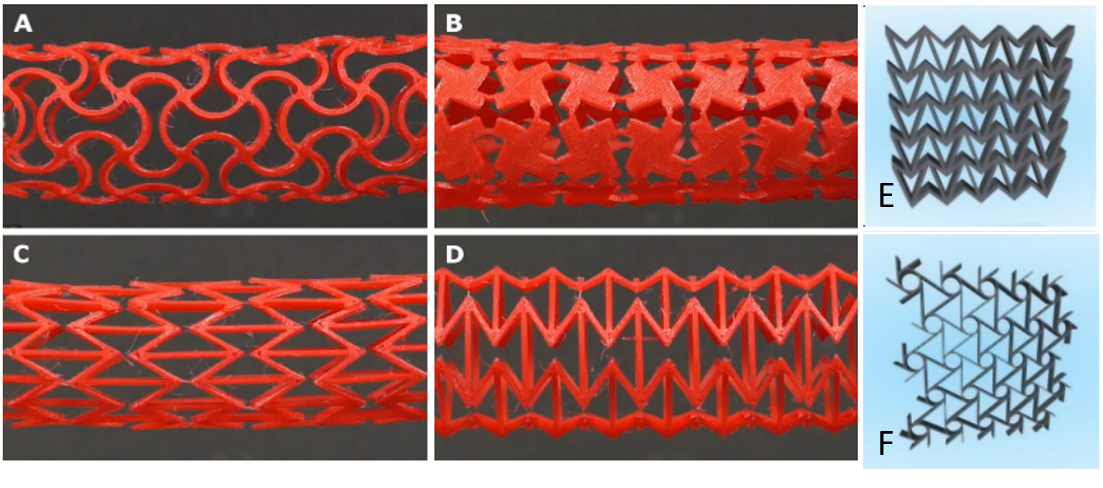
\includegraphics[scale=0.5]{ImageIntro/mailleAuxs.png}
\caption{ Exemples de mailles auxétiques (source : A,B,C,D \cite{Simons2019}; E,F \cite{AlvarezElipe2012})}
\label{fig:maillesAux}
\end{figure}
    
    Il existe néanmoins plusieurs manière d'incorporer celle-ci. En effet, il est possible d'obtenir de telles propriétés  par l'ajout d'un squelette externe à la chambre \cite{Sedal2018} \cite{Karnessis2013} (figure \ref{fig:Exemplescomposition} a, c). Alors, c'est l'ensemble de la chambre et du squelette qui induit le comportement auxétique. Dans d'autres cas, un deuxième matériaux viens renforcer la structure de la chambre elle-même pour laquelle certaines propriétés sont recherchées \cite{Pfeil2018} (figure \ref{fig:Exemplescomposition} b). Le renfort est alors constitué d'un matériau au module d'Young plus élevé (2 GPa contre quelques MPa pour \cite{Pfeil2018}) que celui utilisé pour réaliser la chambre, de la même nature que le squelette externe utilisé dans le premier exemple. Le renfort prend la forme d'un squelette interne constitué d'une répétition de tels motifs. Enfin, il est possible de créer des mousses avec des propriétés auxétiques. Ces propriétés sont alors acquises grâce à la structure microscopique de ces mousses \cite{Critchley2013}.
    
\begin{figure}[ht!]
\centering
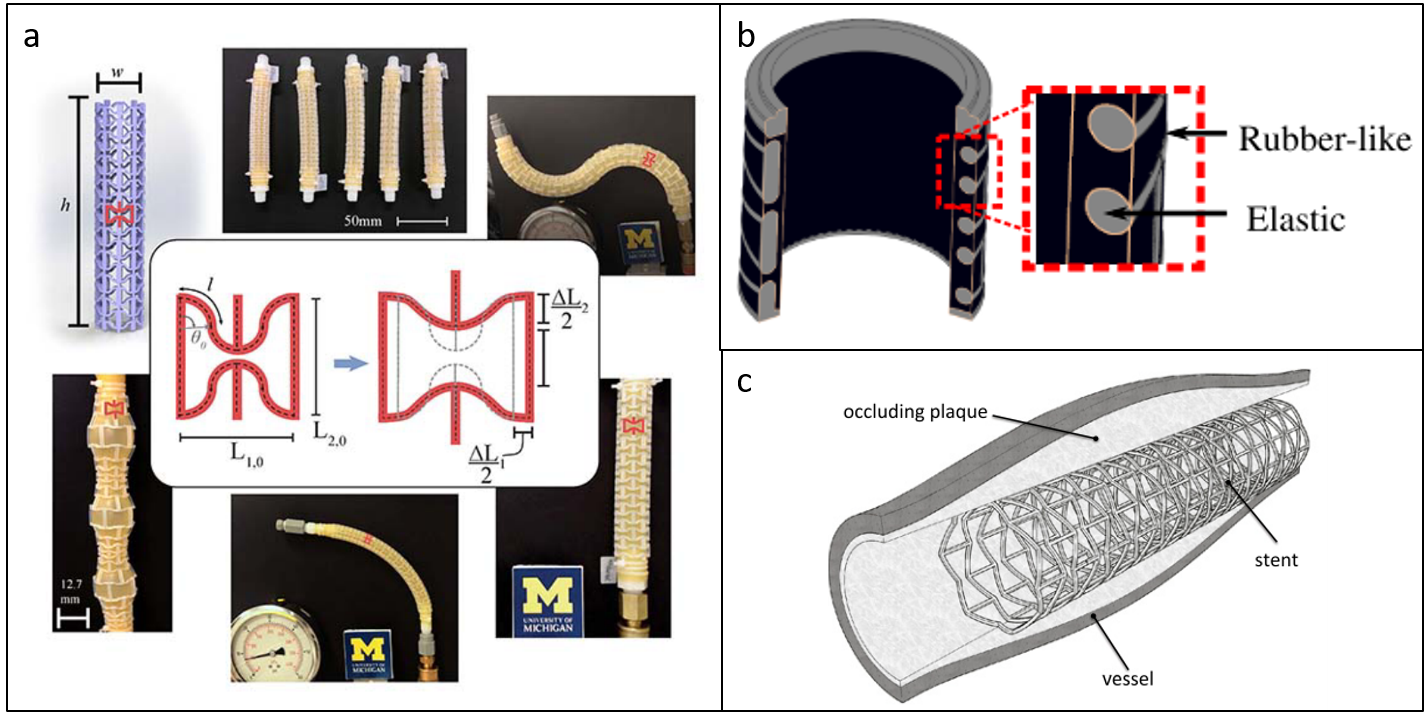
\includegraphics[scale=0.5]{ImageIntro/StructuresAux.png}
\caption{ Exemple d'intégration d'une maille auxétique dans un système (source : a, \cite{Sedal2018}; b, \cite{Pfeil2018}; c, \cite{Karnessis2013};)}
\label{fig:Exemplescomposition}
\end{figure}

    L'utilisation de ces structures est diverses. Certains en font des chambres pneumatiques qui s'allongent sous l'action d'une pression en leurs seins \cite{Pfeil2018}. D'autres se servent de ces structures pour guider un mouvement en adaptant la maille le long de l'actionneur \cite{Sedal2018}. Alors, l'actionneur linéaire devient capable d'actionner linéairement sur n'importe quelle ligne. Il est également possible d'utiliser ces structures en renfort devant certaines déformations comme le vrillage \cite{Karnessis2013}.
    
    \subsection{Actionneurs renforcés par fibres}
    
    Les actionneurs à chambres renforcées de fibres forment une autre classe de systèmes utilisés en mécanique et qui peuvent entrer dans la définition vue en introduction de cette partie. Ce sont en effet des actionneurs pneumatiques dont la chambre qui subit la mise sous pression est un matériau composite qui contient un élastomère autour d'un renfort en fibre dont l'agencement régit les caractéristiques de cette même chambre \cite{Sedal2018a} \cite{Connolly2017} \cite{Takashima2010} \cite{Polygerinos2015} \cite{Lambert2016} \cite{Chou1996} \cite{Science} \cite{Zhang2012} \cite{Doumit2009} \cite{Daerden2002} \cite{Ranzani2016} (figure \ref{fig:chamberFiberEx}). 

\begin{figure}[ht!]
\centering
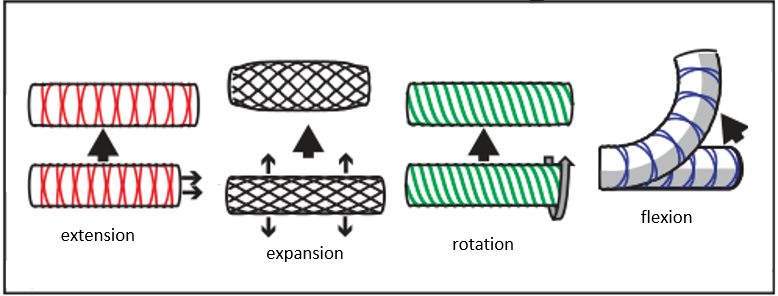
\includegraphics[scale=0.8]{ImageIntro/chamberFiber.png}
\caption{ Exemple de cinématiques possibles avec des chambres pneumatiques renforcées par une fibre (source : \cite{Connolly2017})}
\label{fig:chamberFiberEx}
\end{figure}

    Il est possible aussi de constituer un actionneur avec une cinématique particulière en ayant, de manière séquentielle, un actionneur avec un renfort en fibre dont la forme varie le long de celui-ci \cite{Connolly2017}. Alors, des cinématiques proches de ce qu'un doigt peut accomplir sont accessibles. Cela donne accès à des possibilités de cinématiques particulièrement intéressantes.
    
    L'actionneur pneumatique à chambre renforcée de fibre que la littérature scientifique cite dans de nombreux articles est le muscle artificiel de mac Kibben (figure \ref{fig:stimIRM}) développé dans la fin des années 1950, précurseur dans son domaine \cite{Lambert2016} \cite{Takashima2010} \cite{Daerden2002} \cite{Doumit2009} \cite{Zhang2012} \cite{Chou1996}. Celui-ci possède néanmoins un désavantage certain. La rigidité transversale du muscle artificielle de mac Kibben n'est pas aussi élevée que dans le cas d'une chambre auxétique avec armature rigide. Le guidage des axes actionnés n'est donc pas un aspect pris en compte par cet actionneur.

\section{Modélisation et simulation}
    
    Les différentes techniques utilisées pour modéliser le comportement d'une structure auxétique ou d'une chambre renforcée par fibre sont diverses. Néanmoins, étant basée sur des recherches récentes, car appliquées au domaine de la soft robotique, il n'y a pas d'approche standard à un problème de modélisation de telles structures.
    
    \subsection{Méthodes de conception}
    
        La conception de structures auxétiques et de chambres renforcées par fibres représentent un problème de taille. La multitude de paramètres optimisables et la nature des matériaux mis en jeu rendent celle-ci complexe. Néanmoins, deux méthodes principales sont présentes dans les papiers de la littérature sur le sujet \cite{Sedal2018} \cite{Sedal2018a} \cite{Connolly2017} \cite{AlvarezElipe2012} \cite{Naboni2015} \cite{Karnessis2013} \cite{Chou1996} \cite{Doumit2009} \cite{Polygerinos2015} \cite{Pfeil2018}: l'utilisation d'un modèle analytique et la modélisation par éléments finis.

        Dans le cadre de la modélisation analytique du système, les auteur cherchent à décrire le comportement macroscopique de la chambre à partir des caractéristiques du tissage ou du maillage. Par exemple, la maille en nid d'abeille renversé a déjà été paramétrée \cite{Karnessis2013} \cite{Pfeil2018} (figure ). Les auteurs en déduisent un comportement global et peuvent ainsi en prédire le comportement. Il est néanmoins important de faire remarquer que, dans la cas de la paramétrisation mise en place figure \ref{fig:paramMailleNid}, le nombre de paramètres utilisés n'est pas égal au nombre de paramètres indépendants de la chambre. En effet, seul 7 des 9 paramètres sont indépendant. La conception de cette chambre repose donc sur une optimisation sur 7 paramètres.

\begin{figure}[ht!]
\centering
\centerline{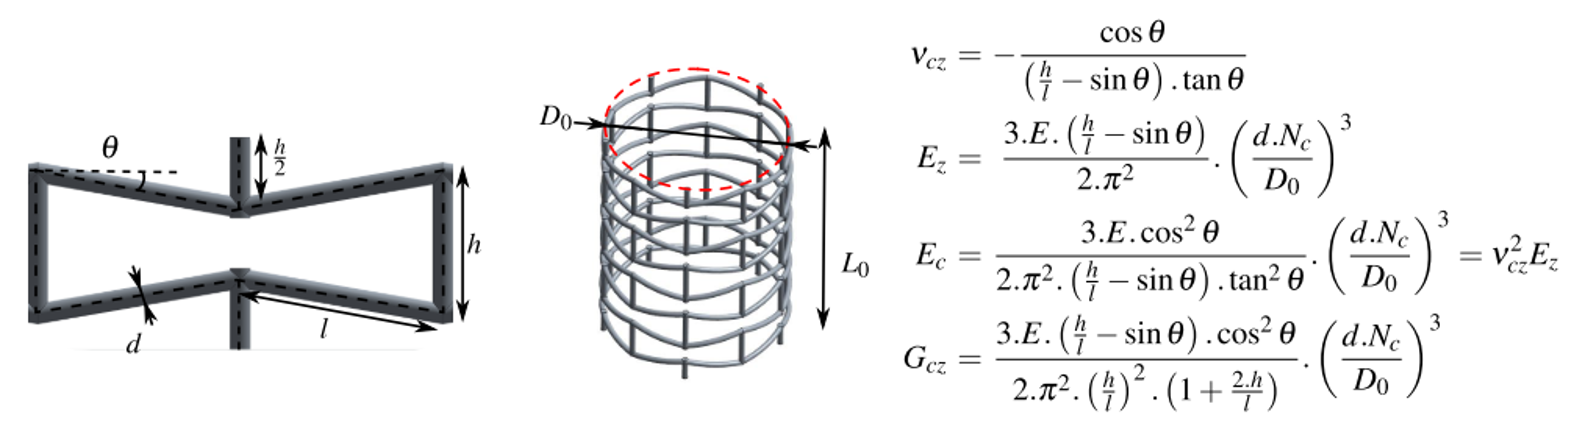
\includegraphics[scale=0.45]{ImageIntro/paramMailleNid.png}}
\caption{ Paramétrisation de la maille en nid d'abeille avec Nc le nombre de mailles sur le tour du cylindre et Nv le nombre de maille sur l'axe, E le module d'Young du matéraiux de la maille (source : \cite{Pfeil2018})}
\label{fig:paramMailleNid}
\end{figure}

        La modélisation analytique n'est pas la seule technique employée par les chercheurs. En effet, devant la complexité de la mise en place d'un modèle analytique, certains préfèrent baser leurs études sur des modèles de simulation par éléments finis \cite{AlvarezElipe2012} uniquement. Néanmoins, il est plus courant de voir l'utilisation des deux méthodes pour la validation de l'un et de l'autre. En effet, dans le cas où les deux méthodes prédisent le même comportement alors qu'elles ne reposent pas forcément sur les mêmes hypothèses, alors, ces modèles sont validées et chacun permet d'apporter des éléments supplémentaire à l'étude \cite{Karnessis2013}.
        
        De plus, certains proposent des outils d'optimisation géométrique de maille basé sur des outils de simulation afin d'obtenir un comportement voulu \cite{Schumacher2018}. La méthode se base sur le comportement voulu et sur le comportement de la maille élémentaire fournie en entrée pour faire varier celle-ci grâce à des outils de simulation et d'optimisation. 
        
        Enfin, d'autres utilisent l'expérimentation pure pour analyser le comportement de chambres définis initialement \cite{Simons2019} \cite{Takashima2010} (figure \ref{fig:maillesAux} , A,B,C,D tiré de \cite{Simons2019}). Néanmoins cette méthode est critiquable dans la mesure où elle n'investit qu'un solution d'un modèle qui lui est général. Par contre cela permet de prendre des directions particulières de modélisations dans le cas où certains phénomènes sont constatés comme l'utilisation de modèles hyper-élastiques ou la prise en compte de non linéarités particulières du système.

    \subsection{Méthodes de validation des caractéristiques}
        
        La conception d'un système prend en compte la validation expérimentale des performances attendues par la réalisation de la chambre dont le modèle fut établie précédemment. Cette étape est cruciale pour convaincre des performances du modèle construit et est mis en place dans bon nombre d'études du domaine \cite{Sedal2018} \cite{Sedal2018a} \cite{Polygerinos2015} \cite{Connolly2017} \cite{Naboni2015} \cite{Doumit2009}. \\
        
        Néanmoins, il est vrai que certains n'ont pas pris le temps de réaliser une validation expérimentale. Cela peut venir du fait que cette étape est longue et complexe si le champ des éléments à valider est trop grand car l'étude investit des modèles éléments finis en grande quantité \cite{AlvarezElipe2012}. Dans le cas de \cite{Karnessis2013}, l'étude ce base sur des non linéarités constatées expérimentalement et la simulation vient étudier ces phénomènes, de même qu'un modèle analytique. Dans ce cas, la validation expérimentale a déjà eu lieu, elle n'a pas été parfaite et une étude supplémentaire permet de faire une adaptation de la simulation. Néanmoins, dans le cas d'une modélisation qui ne tient pas compte de résultats expérimentaux précédents, la validation expérimentale est une étape clef dans la conception d'une nouvelle chambre auxétique ou d'une chambre renforcée de fibres. \\
        
        La fabrication de telles structures représente néanmoins un obstacle à cette dernière étape et il est pertinent de rechercher la combinaison de procédé et de matériau qui permettra une telle fabrication.
        
\section{Matériaux et procédés} 

    Comme évoqué précédemment, la fabrication des chambres auxétiques et des chambres renforcées par fibres sont complexes. La difficulté repose sur les géométries mises en jeu. Certains procédés de fabrications ne serait, par exemple, pas des méthodes appropriées pour la réalisation de chambre en matériaux composites. C'est pourquoi cette partie se focalise sur deux méthodes de fabrications, une méthode de fabrication additive et plusieurs méthodes de moulage.
    
    \subsection{Fabrication additive par photo-polymérisation}
    
    \qquad Comme décrit dans la partie 2.2 précédente, le procédé de fabrication par dépôt de photopolymère permet de réaliser des pièces en petites séries et de créer des géométries que les autres procédés ne peuvent réaliser. Néanmoins, ce procédé a des limites. En effet, les matériaux mis en formes n'ont pas les propriétés du matériaux initialement utilisé. Le procédé dégrade celle-ci. La communauté scientifique s'accorde sur le fait que beaucoup de paramètres influe sur les propriétés mécaniques des pièces formées. La position dans le plan de travail (\cite{Herdiana2013}, \cite{Gay2015}), l'orientation de fabrication (\cite{Beltran2015}, \cite{Gay2015}), la densité et le motif de remplissage (\cite{Barnik2019},\cite{Yang2019}). \newline\newline
    
    \quad  Parmi les propriétés altérées par le procédé de fabrication, on retrouve le module d'Young qui, en plus de diminuer globalement, devient anisotrope à cause de la fabrication couche par couche dans une direction donnée. Néanmoins, dans le cadre de la photo-polymérisation, il est envisageable de considérer ce phénomène comme secondaire dans la mesure où l'on dépose une couche de photo-polymère sur une couche qui n'est pas complètement polymérisée. Alors,le tout forme un ensemble  homogène \cite{Herdiana2013}. Néanmoins, la résistance à la fatigue et à la rupture sont grandement impactés par le procédé car chaque couche est une potentielle amorce de rupture (figure \ref{fig:coupeTango}) \cite{Barnik2019}. \\
    
\begin{figure}[ht!]
\centering
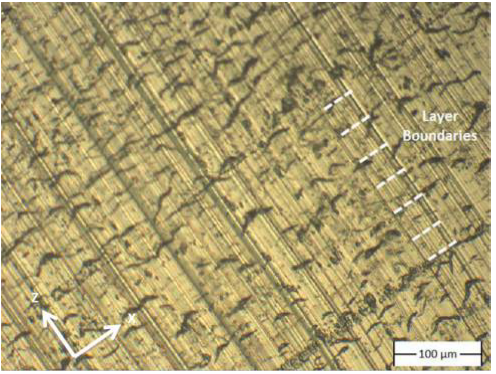
\includegraphics[scale=0.65]{ImageIntro/coupePolyjet.PNG}
\caption{ Vue microscopique d'une découpe de TangoBlack mis en forme par impression 3D Polyjet (source : \cite{Moore2015}) }
\label{fig:coupeTango}
\end{figure}
    
   \quad De plus,le fait que le procédé mette en forme les deux matériaux dans la même étape fait apparaître des problèmes d'interfaces entre ceux-ci. Une interface entre ces deux matériaux devient alors une amorce de rupture potentielle supplémentaire ce qui réduit la résistance de la pièce à la fatigue et à la rupture (figure \ref{fig:essai}) \cite{Moore2015} \cite{Vu2014}. 
    
\begin{figure}[ht!]
\centering
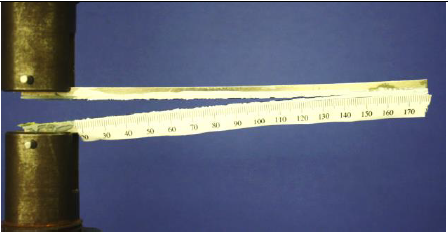
\includegraphics[scale=1]{ImageIntro/EssaiInterfaceTBVW.PNG}
\caption{ Essai réalisé pour étudié l'interface en les deux matériaux TangoBlack et VeroWhite (source : \cite{Vu2014})}
\label{fig:essai}
\end{figure}
    
    \subsection{Moulage}
    
    Il est aussi possible de réaliser ces structures particulières à l'aide de plusieurs étapes. La première serait un usinage de la chambre auxétique ou un tissage du renfort de la chambre. La seconde étape reposerais sur le moulage d'un matériau, comme un élastomère, autour de la structure. Cette méthode ayant déjà été réalisé par d'autres pour fabriquer de telles structures \cite{Polygerinos2015}. La famille des procédés de moulage est très grande \cite{Schmitt2018}. Il est possible d'y retrouver de nombreux procédés qui ont leurs avantages et inconvénients (figure \ref{fig:moulageTableau}). Il est pertinent de s'intéresser aux méthodes de mises en formes de la robotique souple dans notre cas étant donné la nature des matériaux à mettre en forme. Dans cette catégorie, trois méthodes principales apparaissent. Néanmoins, certaines problématiques restent communes à l'ensemble des techniques de moulage comme le fait que le surmoulage impose le maintient de l'élément surmoulé dans le moule ou encore l'adhésion en le matériau moulé et l'élément surmoulé \cite{Schmitt2018}.
    
        \subsubsection{moulage par injection}
        
            Le moulage par injection est un moulage très utilisé dans le domaine industriel (https://www.husky.co/FR-FR/) et est utilisé pour la réalisation de robot souples\cite{Marchese2015} \cite{Polygerinos2015}. Ce procédé est très adapté à la grande série car l'usinage des moules est une étape onéreuse. Néanmoins, avec les méthodes de fabrication additive \cite{Marchese2015} \cite{Polygerinos2015}, ce coût peut être fortement réduit. Il est néanmoins nécessaire de prendre en compte des aspects particuliers des polymères moulés. En effet, ceux-ci doivent être dégazés. D'autres procédé permettent de ne pas se soucier de cette problématique
        
            
\begin{figure}[ht!]
\centering
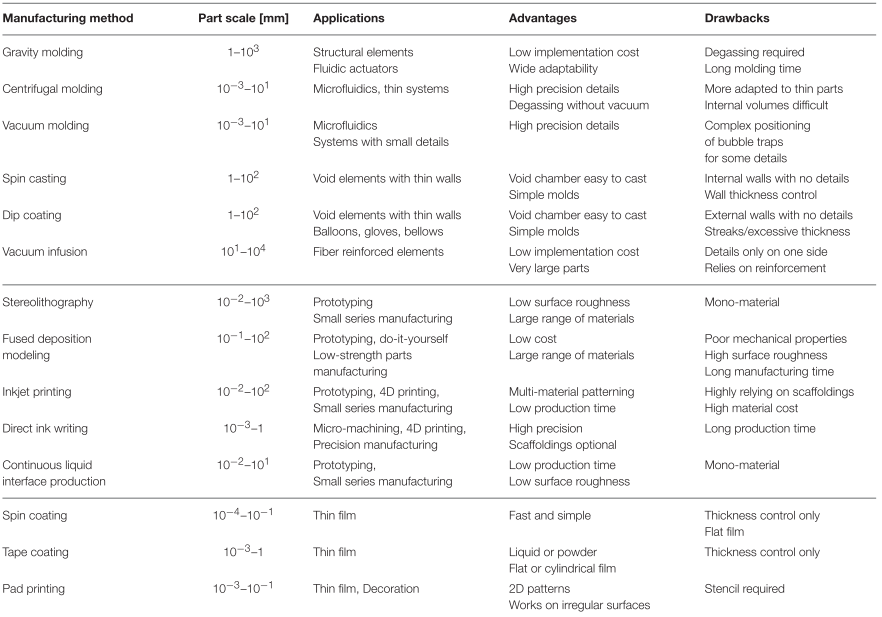
\includegraphics[scale=0.5]{ImageIntro/tableauMoulage.PNG}
\caption{ Tableau recensant les méthodes étudié dans l'article source (source : \cite{Schmitt2018})}
\label{fig:moulageTableau}
\end{figure}
            
        \subsubsection{Lithographie}
        
        Dans le domaine de la soft robotique, la lithographie s'inspire des premiers âges de l'imprimerie \cite{Marchese2015}. Un moule plan et avec des éléments de reliefs souhaités sur le robot (figure \ref{fig:lithographie}) sert de support au matériau à mettre en forme. Le matériau est coulé sur le plan pour que les différentes parties soient collées à la fin. Cette dernière étape peut être source de désagréments comme des fuites ou des ruptures inopinées. Le procédé de mise en forme plan, et de collage ensuite, impose des contraintes de conception particulières comme des formes démoulables ou encore des questionnements sur la possibilité que des bulles d'air reste en places et fragilisent l'objet final \cite{Marchese2015}.
        
\begin{figure}[ht!]
\centering
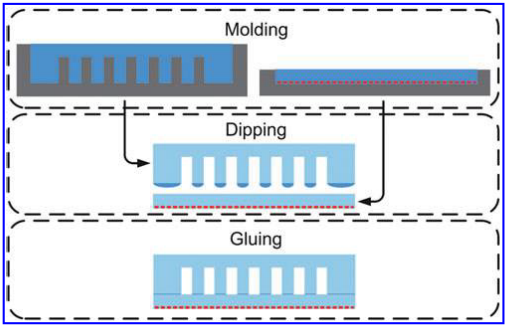
\includegraphics[scale=0.5]{ImageIntro/lithograp.PNG}
\caption{ Présentation du procédé de lithographie (source : \cite{Marchese2015})}
\label{fig:lithographie}
\end{figure}

\subsubsection{moulage par centrifugation}

            Le procédé de moulage par centrifugation figure permet de mettre en forme des formes complexes comme des cavités fermées en un minimum d'étape \cite{Zhao2015} (figure ). Cette méthode de fabrication se rapproche de la lithographie. Dans le cas présent, la gravité est remplacée par la force centrifuge. A nouveau, des problématiques de démoulage se posent mais cette méthode permet, notamment, de dégazé les polymères mis en formes par cette méthode sans étape supplémentaire et sans mise sous vide \cite{Schmitt2018} \cite{Mazzeo2013}. Le désavantage principal de cette méthode est que l'épaisseur moulé n'est pas garantie et contrôlée.
            \cite{Vu2014}

\begin{figure}[ht!]
\centering
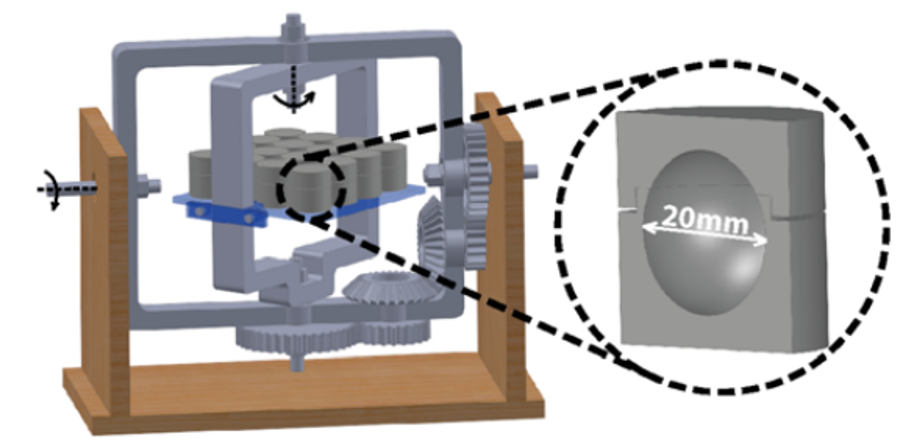
\includegraphics[scale=0.5]{ImageIntro/centrifugationMoulage.png}
\caption{ Présentation du procédé de moulage par centrifugation (source : \cite{Zhao2015})}
\label{fig:centrifugation}
\end{figure}
        
        
        
\section{Perspectives}

    L'objectif est maintenant d'utiliser le système existant dans la conception d'un nouveau système avec ses objectifs d'actionnements propres et ses performances attendues. Il faudra utiliser le contenu précédent pour réaliser un certain nombre de choix quant à la démarche de conception, le choix de la structure du système et son procédé de fabrication.



\bibliographystyle{plain} % We choose the "plain" reference style
\bibliography{Biblio} % Entries are in the "refs.bib" file




\listoffigures

\end{document}